\chapter{Air- and Rail-Transport}
\label{ch:air}
% ##################################################################################################################

\hfill \textbf{Author:} Dominik Grether

\begin{center} 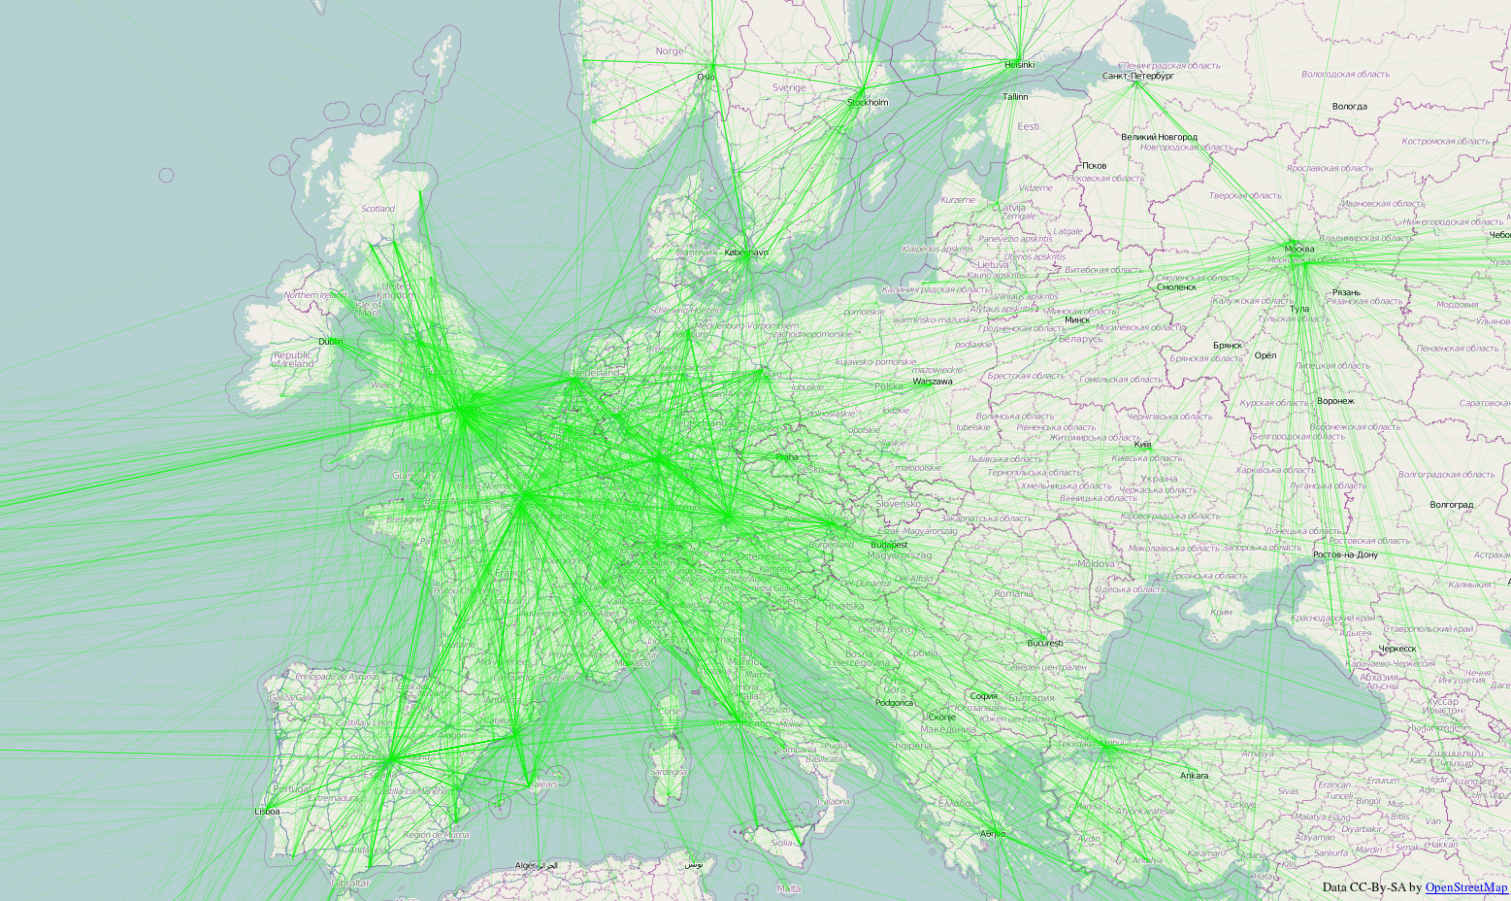
\includegraphics[width=0.6\textwidth, angle=0]{extending/figures/air/air_network_europe_osm} \end{center}

\editdone{This text has undergone the professional edit. Please no grammatical changes anymore! They are most-probably wrong.}

\createStandardInformationBasic{\lstinline|playground.fuerbas.air| package}{No standard invocation.}{No standard config.}{\citet{GretherFuerbasNagel2013FlightTechnologyPROCEDIA,Grether2014PhD}}
\joschka{Kai: Hier wäre m.E. gar nichts Standard - vielleicht nehmen wir den obigen Eintrag einfach komplett raus und lassen nur die Referenz auf die Publikation?}
% ##################################################################################################################
This chapter discusses simulation of air- and rail-transport technology and passengers using \gls{matsim}. 
There is no great difference in overall travel times between middle-range rail and air transportation. 
Airports and railway stations are affected by capacity and opening time constraints. 
For passengers and goods, geospatial location is an important property. 
Both modes, but especially air transport, are faced with difficult capacity restrictions at fixed departure times. 

This chapter discusses how \gls{matsim} can be applied to capture these constraints and how interaction between passenger demand and constraints on technology supply can be modeled. 
The public transit model of \gls{matsim} (Chapter~\ref{ch:pt}) is applied. %public transit vehicles and stops. 
Airports and aircraft are microscopically modeled the same way as bus stops and buses. 
Passengers are represented microscopically as multi-agent demand for air transportation. 
Their choices of transport mode, routes, and departure time are restricted by the air transport technology simulation model's capacity. 
The modeling of rail transport is based on \gls{teleportation}. 
With appropriate data, the modeling approach for air transport could also be applied to rail transport \citep{Quick2012BARailTraffic}.  

The modeling of technology and demand is sketched in Section~\ref{sec:air_rail_scenario}. 
On the basis of simulation results for a pure air transport model, rail transport is added and effects of mode choice are presented (Section~\ref{sec:air_rail_results}). 
Section~\ref{sec:air_rail_discussion} then interprets simulation results and highlights some modeling aspects requiring further study. 
The choice set generation and plans removal algorithm of \gls{matsim} is discussed in detail; that is also the subject of Section~\ref{sec:future-of-scoring-function}. 
Modeling, results, and studies of this chapter present the highlights of \citet[][Chapter~6, pp.~119]{Grether2014PhD}, in more detail.   

% ##################################################################################################################
\section{Air Transport Scenario}
\label{sec:air_rail_scenario}
% ===========================================================================================
\subsection{Modeling \& Simulation of Air Transport Technology}
\label{sec:modeling-of-technology}
%
%\begin{figure}[t]
	%\begin{minipage}{0.5\linewidth}
				%\centering
			%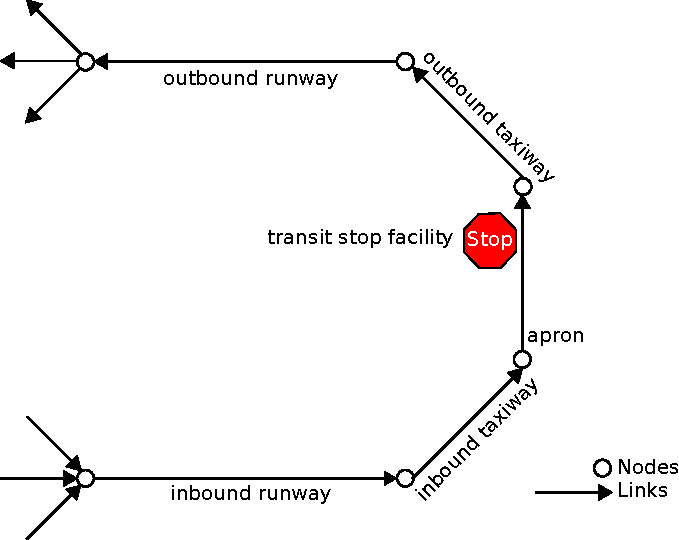
\includegraphics[width=0.9\textwidth]{extending/figures/air/sf_flight_model_airport.pdf}
		%\vspace{1.3cm}
%
			%%\scriptsize
			%\footnotesize
			%\begin{tabular}{@{}lrrr@{}}
				%Linktype & Count & Length [m] & Speed [km/h] \\
				%\hline
				%Runway   	& 2					& 1500		& $length \cdot c_{flow} $  	\\ % former value 220
				%Taxiway   	& 2					& 500		& 20  	\\
				%Apron   		& 1					& 500		& 20  	\\
				%\end{tabular}		
				%\vspace{1.4cm}
				%\caption{Airport layout and characteristics}
				%\label{fig:matsim_airport}
	%\end{minipage}
	%\begin{minipage}{0.5\linewidth}
		%\centering
		%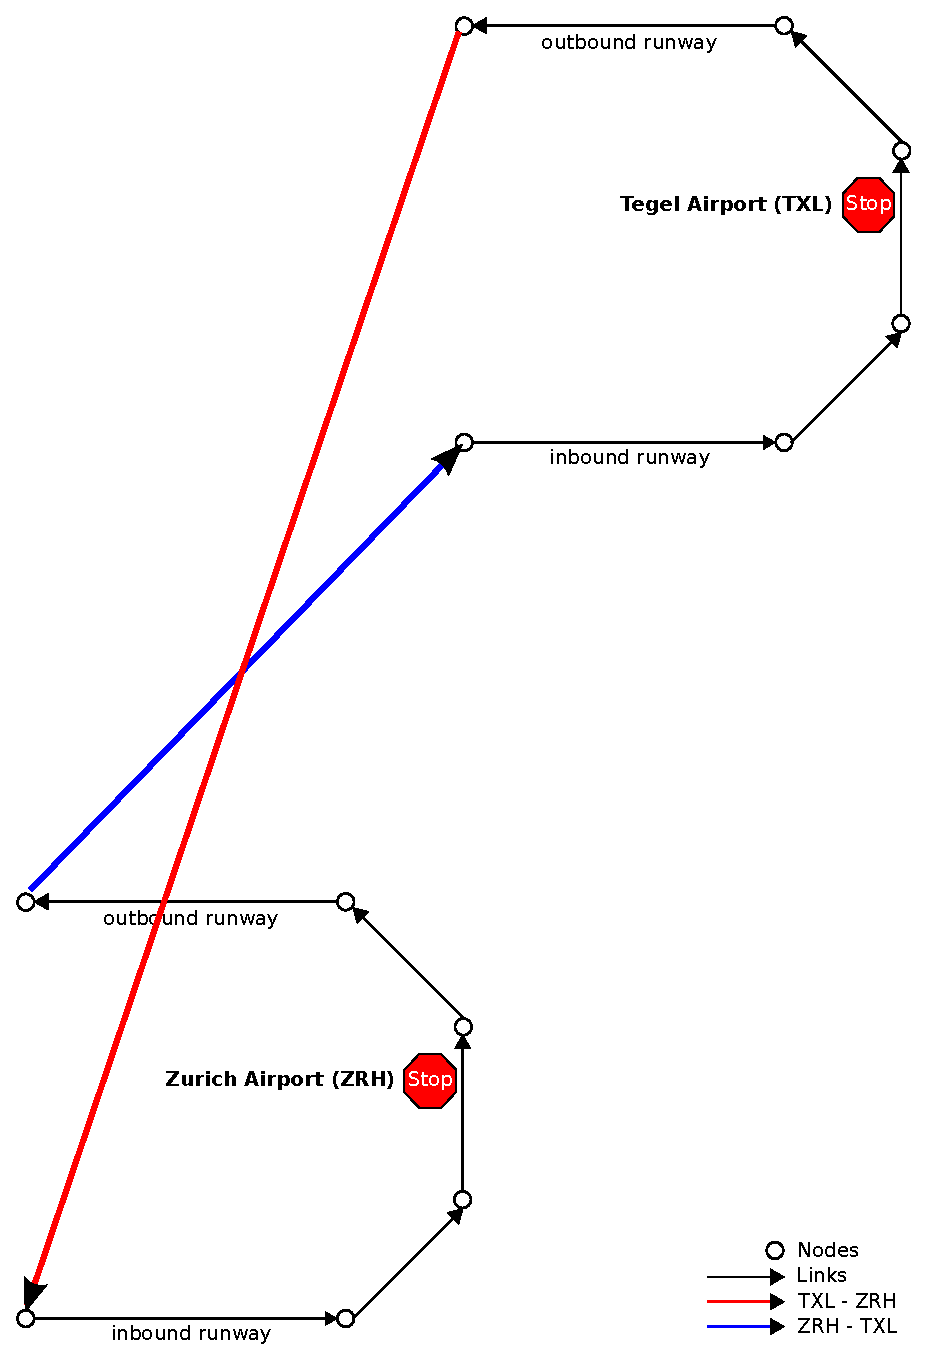
\includegraphics[width=0.9\textwidth]{extending/figures/air/sf_airport_network_no_slide.pdf}
		%\caption{Network layout}
		%\label{fig:matsim_network_model}
	%\end{minipage}
	%\caption{Layout of the air network, Source:~\citet{Grether2014PhD}}
	%\label{fig:air_network}
%\end{figure}
%
% ------------
\createfigure%
{Layout of the air network}%
{Layout of airports in the air transport network: In- and outbound runways are modeled by separate links connected by taxiways and a link representing the apron. There the transit stop facility is attached}%
{\label{fig:air_airport}}%
{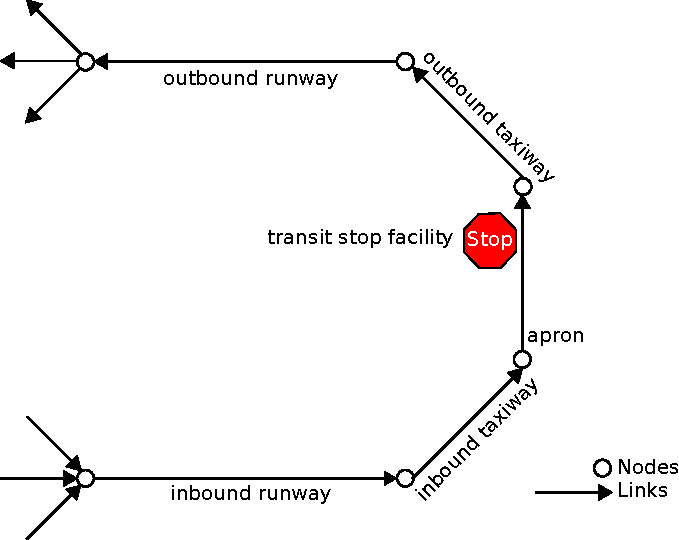
\includegraphics[width=0.8\textwidth]{extending/figures/air/sf_flight_model_airport.pdf}}%
{\citet{GretherFuerbasNagelFlightTechnology}}
% ------------
%
%\createtable%
%{Airport layout and characteristics}%
%{Airport layout and characteristics}%
%{\label{fig:matsim_airport}}%
%{%
%  \begin{tabular}{lrrr}
%		Linktype & Count & Length [m] & Speed [km/h] \\
%		\hline
%		Runway   	  & 2					& 1500	& $length \cdot c_{flow} $  	\\ % former value 220
%		Taxiway   	& 2					& 500		& 20  	\\
%		Apron   		& 1					& 500		& 20  	\\
%	\end{tabular}	
%}%
%{}
%
% ------------
\createfigure%
{Network layout}%
{Layout of airways in the air transport network: each airport pair is directly connected by two airway links, one for each flight and direction}%
{\label{fig:air_network_model}}
{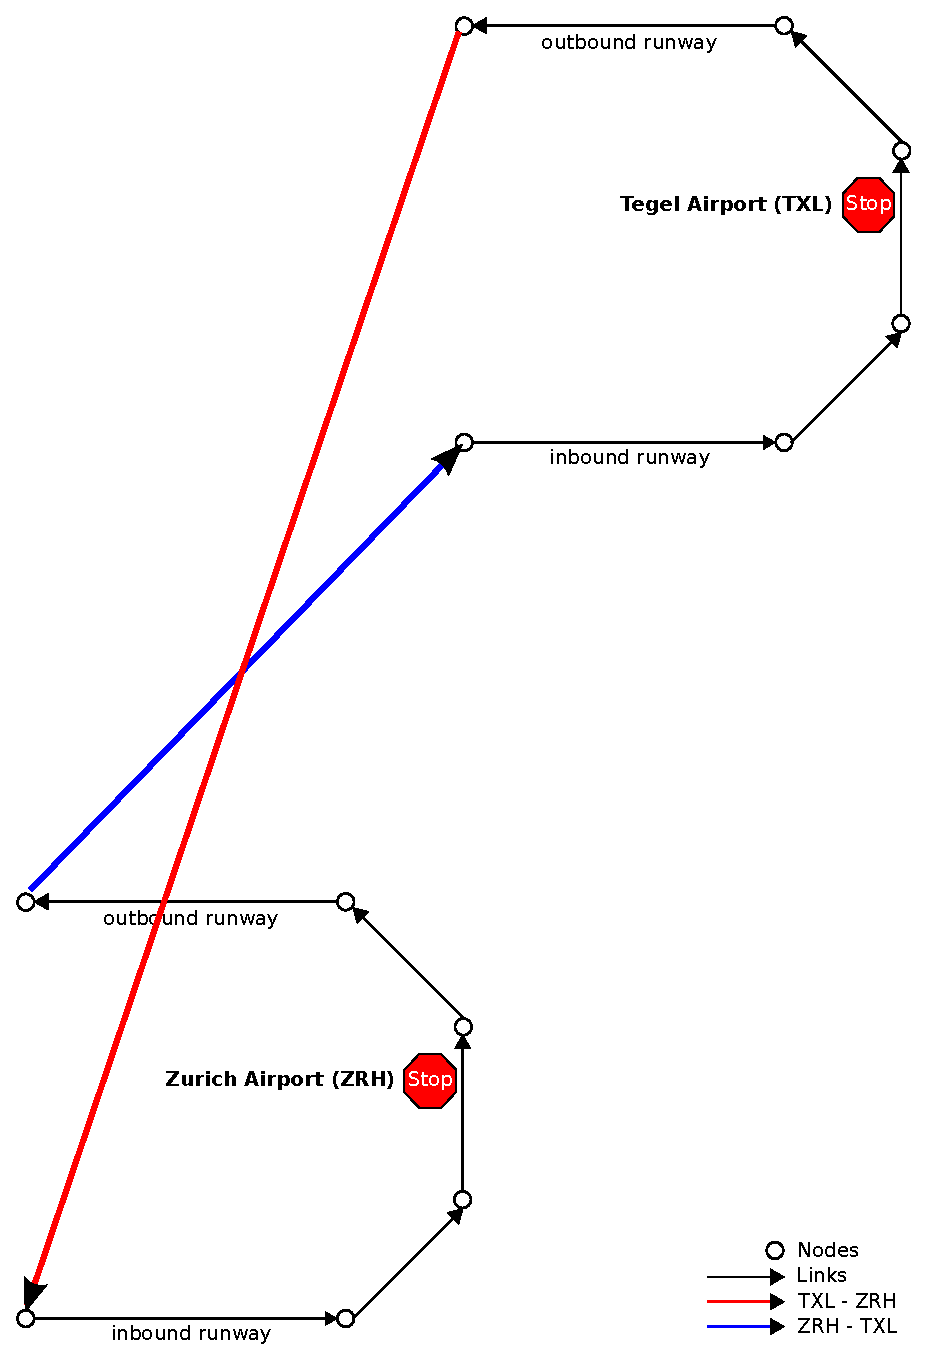
\includegraphics[width=0.8\textwidth]{extending/figures/air/sf_airport_network_no_slide.pdf}}%
{\citet{GretherFuerbasNagelFlightTechnology}}
% ------------

%\mnote{OAG}
The air traffic technology model uses data provided by OAG \ah{glossary} Aviation.%
\footnote{\url{www.oagaviation.com}, last access 08.08.2012}
Relevant data for schedule and network generation is taken from the September 2009 OAG \ah{glossary} data, using all flights departing on a Tuesday, taking each specific flight number into account only once.
This may not always result in complete flight cycles, \eg when the outbound and inbound flight operate on different days of the week. 
Compared to using all flights of an entire week, the network may be incomplete, as certain destinations are only served on specific days.

%\mnote{Network}
The air network modeling aims at a simulation with \gls{matsim}.  
The network consists of airports, each showing an identical layout and point-to-point connections in between. 
Every runway is solely used either for inbound or outbound flights, with taxiways connecting the runways to the apron. The latter accommodates a transit stop, \ie the terminal, where flight movements originate and terminate (Figure~\ref{fig:air_airport}). 
Each airport pair is directly connected by airway links, one for each flight and direction of travel (Figure~\ref{fig:air_network_model}). 
Maximum speed on any of these links is calculated based on distance and flight duration provided by OAG \ah{glossary}. 
Times for taxi, take-off, and landing are also taken into account, \ie flight duration is reduced by the time needed from push-back to airborne before the maximum speed for an airway link is calculated.
Each flight has an individual link that could be interpreted as route, each possessing individual characteristics. 
Figure~\ref{fig:matsim_air_network_eu} shows parts of the network for European air traffic.
%
% ------------
\createfigure%
{European air network}%
{European air network with country borders in the background (country borders~\textcopyright~\url{openstreetmap.org})}%
{\label{fig:matsim_air_network_eu}}%
{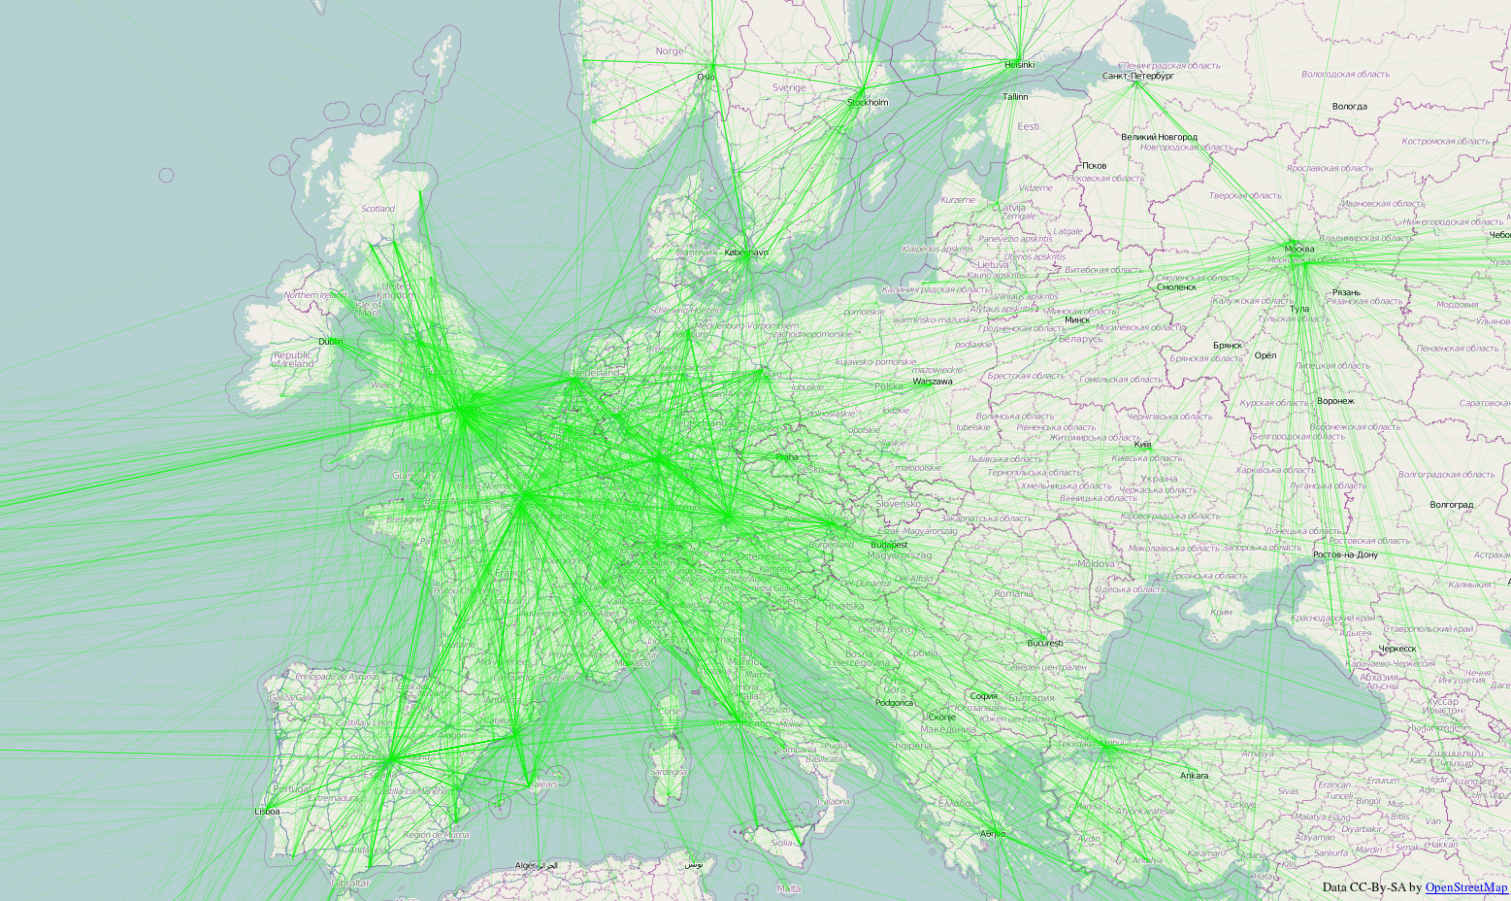
\includegraphics[width=0.99\textwidth, angle=0]{extending/figures/air/air_network_europe_osm.png}}%
{\citet{GretherFuerbasNagelFlightTechnology}}

% ------------

%\mnote{Flight Schedule}
Flight schedules are taken from the OAG data and translated to a \gls{matsim} transit schedule containing information about each line, route, and departure. 
For each airline offering a connection between two airports, a transit line is generated. 
A transit route, which represents the route on the air traffic network, is created for each flight offered by this airline. 
%The route contains the links belonging to the airport representation plus the specific link for this flight connecting the airports' out- and inbound runway. 
Mutual interferences of aircrafts en-route are not included in the studies presented in this chapter.
%Tab.~\ref{tab:number_of_flights} lists the number of (not included) airports, direct origin-destination (O-D) connections and flight movements for three different area pairs.

%\mnote{Vehicles}
To represent individual aircraft in the simulation, transit vehicles are created on the basis of OAG data. 
IATA aircraft codes, operating airlines, and seating capacities are reflected in the respective aircraft representation for every flight. 
Information about boarding times, \ie passenger flow per door over time, is not available, but could be set for each aircraft type. 
One aircraft per flight is generated, thus delays resulting from a delayed incoming aircraft are not modeled.
Accordingly, no aircraft rotations and vehicle trip chains are implemented at this time. 
The maximum velocity of each aircraft is set to twice sonic speed, since speed limitations are set for each network airway link. 

% ===========================================================================================
\subsection{Passenger Demand}
%\mnote{Passengers, Synthetic Population}
As soon as the technology side of air transport is modeled, passenger demand simulation can begin. 
The passenger demand for trips in Germany created and used for the results of this section is based on \gls{od} data of DESTATIS.% 
\footnote{\url{destatis.de}, Fachserie~8 Reihe~6, last access 10.09.2012}.
% 
For each \gls{od} pair and trip a virtual person is created.
Each virtual person performs two activities, one at the origin and the other at the destination airport. 
Both activities are of same type, thus time spent performing both activities is accumulated before it is evaluated by the utility function according to Section~\ref{sec:charyparnagel}. %equation (\ref{eq:utility_v_perf}). 
A typical duration, $t_{typ,q}$, of 21\,hours is set for this activity type. 
The time virtual persons arrive at the origin airport and start waiting for a connection is drawn randomly from a uniform distribution in 04\,am to 6\,pm, UTC. 
This reflects estimated typical opening hours of European airports.
No other time constraints are set, thus the only incentive for virtual persons is to reduce overall travel time and maximize time spent at the activity. 
A flight leg is scheduled between the two activities, connecting origin and destination.
As usual, the demand does not specify if a direct flight from O to D is chosen or the virtual person is on a route containing one or more transfers.
The synthetic population contains 51\,832\,virtual persons, 1\,550\,trips from the original data are neglected as origin and destination are equal.

%\karen{this last sentence doesn't make sense. Please rewrite? Does he mean 'selected' instead of 'neglected'??} 
%\ah{yes, they are neglected as they do within-zone travel}
%

% ##################################################################################################################
\section{Simulation Results}
\label{sec:air_rail_results}
% ===========================================================================================
\subsection{Air Transport}
%\mnote{Parameters}
As a scenario for air transport technology, a coverage model from Europe to world wide destinations is used; 
with the synthetic population, it serves as input for the simulation.
%model with no delays and no effective runway capacity restrictions 
%from 
%\technologyCite~is used.
The assignment of flights to the desired \gls{od} connection, \ie the passenger routing, is calculated by \gls{matsim} 's default public transit routing module.

%\mnote{Simulation Runs}
Each simulation is run for 600\,iterations.
In each iteration, 10\,\% of the virtual passengers may shift their departure time randomly within a 2\,hour interval.
Another 10\,\% may seek a new route, \ie a connection between origin and destination. 
Each passenger chooses from a set of 5\,plans using an \gls{mnl}.
The outcome is stable after 500\,iterations, then departure time choice and routing are switched off. 
For another 100\,iterations only the \gls{mnl} is used by  passengers to select a plan. 
%
% ------------
\createfigure%
{Passengers in aircraft and available seats over time in Germany}%
{Passengers in aircraft and available seats over time in Germany: At any time, there are more seats than passengers. Air transport-only scenario based on O-D data for Germany, iteration~600}%
{\label{fig:2009_passengers_seats}}%
{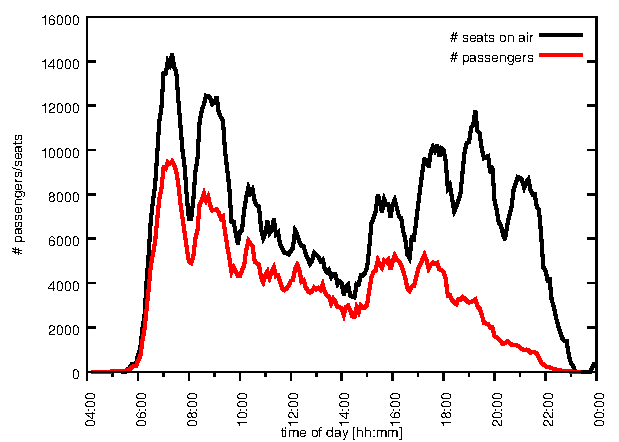
\includegraphics[width=0.99\textwidth, angle=0]{./extending/figures/air/in_vehicle_histogram_flight_1876_it_600.pdf}}%
{}

% ------------

Results are then taken from the output of the 600th iteration. 
Filtered by flights in Germany, Figure~\ref{fig:2009_passengers_seats} depicts passengers in aircraft (red) and seats (black) over time of day
and reveals passengers' tendency to depart early. 

Some passengers fail to reach their destination and are ``stranded''.   
This is unrealistic; only trips within Germany are modeled. These are usually completed within a few hours, with no requirement for an overnight airport stay. 
320\,passengers stranded at the end of the day. 
Getting stranded is not a result of insufficient seating; at any time of day, there are more seats than demand.  
%
There are many reasons why passengers could be stranded in such a situation.
%
Further analysis of the $c_{lineswitch} = 0$ scenario simulation results indicates:
\begin{itemize}\styleItemize
\item 92\,passengers are stranded because there is no seat and no other flight on the same airline later that day, to which they could be shifted.
\item 228\,passengers are stuck at an airport because there is no connection after their departure time 
	between that airport and their destination airport. 
\end{itemize}

Behavioral aspects: neither departing early, nor getting stranded, are explicitly modeled.  

% ===========================================================================================
\subsection{Adding an Alternative Mode}
%\mnote{Simulation Setup}
To gain further insights, in the following a slightly different simulation setup is applied. 
%The additional cost for each transfer is fixed to $c_{lineswitch} = 0$ and has no influence on the model. 
A second option for mode choice is added. 
Each virtual passenger can now choose between the microsimulated air transport options and an alternative mode. 
The alternative mode has no capacity restrictions. 
Passengers traveling with the alternative mode can start directly at their randomly selected departure time. 
The travel time, $tt$, is computed by the \gls{microsimulation}, with an estimation of the beeline distance between the \gls{od} pair $d$ and a velocity $v$, \ie $tt = d / v$.  
This velocity is varied in several simulation runs, \ie $v \in \{100, 150, 200, 250, 300 \} [km/h]$. 
If the alternative mode is chosen, the (dis-)utilities for traveling are calculated accordingly in the scoring.  

%Each person in the synthetic population obtains a second plan employing the alternative mode. 
With this population, the simulation is again run for 600\,iterations. 
As in the previous simulations 10\,\% of the virtual passengers may shift their departure times, while another 10\,\% seek a different route between origin and destination in the air transport network. 
Additionally, further 10\,\% of virtual persons may change mode, \ie they can switch between the air traffic mode and the alternative mode. 
After 500\,iterations all choice modules are switched off; thus, for the last 100\,iterations, passengers use the logit model to select a plan. 

Simulation results for the 600th iteration show that the increasing speed of the alternative mode affects the modal split.  
While for a $v = 100 \, km/h$ the alternative mode is chosen by 1.2\,\% of the passengers, a mode alternative with a speed of 300\,kilometers per hour attracts 15.69\,\% of travelers. 
The number of stranded passengers for the alternative mode with $v = 100$\,kilometers per hour is substantially reduced, from approximately 320 to 67. 
Higher speeds of the alternative mode further reduce the number of stranded passengers. 
Slow speeds of the alternative mode imply dominance of the air transport mode. 
If there is a seat on a flight, travelers receive a higher score than when they use the alternative mode. 
However, travelers risk getting stranded, which can be hard to analyze and interpret. 
The implemented algorithm is also an open issue; if the number of plans per traveler exceeds a threshold of 5, the plan with the lowest score is removed from the plan database. 

% ------------
\createfigure%
{Results with random selector for plan removal, iteration~600.}%
{Passengers waiting for a flight, traveling by plane, or by alternative mode over time of day. 
Air transport and alternative mode scenario for Germany, iteration~600. Results with random selector for plan removal}%
{\label{fig:2009_leg_histogram_modes_psl}}%
{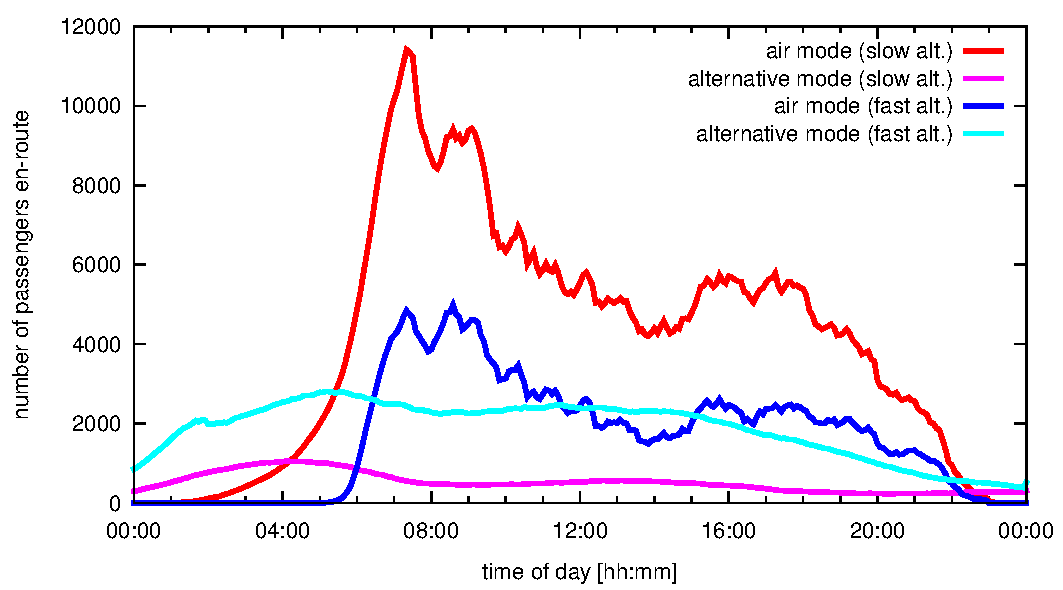
\includegraphics[width=0.99\textwidth, angle=0]{./extending/figures/air/leg_histogram_improved_flight_train_en_route_1893_1897_it_600.pdf}}%
{\citet{Grether2014PhD}}

% ------------
%
\createtable%
{Results with random selector for plan removal, iteration~600. Modal split for different speeds of the alternative mode}%
{Modal split for different speeds $v$ of the alternative mode. % 
Air transport and alternative mode scenario for Germany, iteration~600. %
Results with random selector for plan removal% 
}%
{\label{tab:2009_results_train_modal_split_psl}}%
{%
  \begin{tabular}{@{}l|ccc|ccc@{}}
		$v [km/h]$	& \# air mode  & \# alt.~mode & \# stuck & air mode[\%]  & alt.~mode[\%] & stuck[\%] \\
		\hline 
		100 & 49280 & 2551 & 1 & 95.08 & 04.92 & 00.00\\	%1893 & 600
		150 & 44835 & 6996 & 1 & 86.50 & 13.50 & 00.00\\	%1894 & 600
		200 & 39929 & 11902 & 1 & 77.04 & 22.96 & 00.00\\	%1895 & 600
		250 & 34332 & 17499 & 1 & 66.24 & 33.76 & 00.00\\	%1896 & 600
		300 & 27270 & 24562 & 0 & 52.61 & 47.39 & 00.00\\	%1897 & 600
	\end{tabular}
}%
{}

Instead of this deterministic plan removal, a probabilistic algorithm can be implemented: \eg plans for removal can be selected based on a path size logit model. 
With this modification, simulation runs are repeated. 
%with the same setup as the runs incorporating the alternative mode. 
Figure~\ref{fig:2009_leg_histogram_modes_psl} shows the resulting travel patterns over time for alternative modes at speed 100\,kilometers per hour and 300\,kilometers per hour.  
Traveler distribution on the alternative mode over time of day is quite homogeneous. 
The alternative mode speed increase attracts more passengers, as 
reflected by the modal splits in Table~\ref{tab:2009_results_train_modal_split_psl}. 
At most, one passenger is stranded at the end of day. 

\createtable%
{Random selector results for plan removal, iteration~600. Simulation results including an alternative mode at different speeds $v$}%
{%
Error calculations for different speeds $v$ of the alternative mode. % 
Air transport and alternative mode scenario for Germany, iteration~600. %
Results with random selector for plan removal% 
}%
{\label{tab:2009_results_alternative_mode_psl}}%
{%
  \begin{tabular}{@{}l|cccc@{}}
			$v [km/h]$ & $\sigma^2$ & $\sigma$ & mean rel error  & stuck \\
\hline
 $od_{transfer} - od_{direct}$ &  12640 & 112 & 1.75 & - \\
 \\
 100	& 10367 & 102 & 0.35 &  1 \\	% 1893 & 600
 150	& 13820 & 118 & 0.43 &  1 \\	% 1894 & 600
 200 & 18651 & 137 & 0.56 &  1 \\	% 1895 & 600
 250 & 25291 & 159 & 0.68 & 1 \\	% 1896 & 600
 300 & 36059 & 190 & 0.76 & 0 \\	% 1897 & 600
		\end{tabular}
}%
{}

Simulation results are compared in more detail with DESTATIS data serving as a base for the virtual population.  
Synthetic population is generated based on \gls{od} pairs that may contain transfers ($od_{transfers}$), 
while other DESTATIS data counts the number of passengers on actual direct flights ($od_{direct}$). % (2.2.1).
The latter is used to evaluate model accuracy.
For comparison, number of passengers on direct flights is calculated for each \gls{od} pair ($sim_{direct}$) from the simulation results.
Based on these data sets, the mean square error and the mean relative error are calculated.%
\footnote{
The mean square error $\sigma^2$ is computed as
	$\sigma^2 = \frac{\sum_{i \in OD} (sim_{direct}(i) - od_{direct}(i))^2}{|OD|} \, , $
whereby $|OD|$ denotes the number of \gls{od} pairs, $sim_{direct}(i)$ the simulated passengers on a direct flight between the \gls{od} pair $i$, and $od_{direct}(i)$ the same, but retrieved from data.  
With the same values, the (unsigned) mean relative error for each \gls{od} relation is calculated as
$
\mbox{mean rel error} = \frac{\sum_{i \in OD} |(sim_{direct}(i) - od_{direct}(i))|/ od_{direct}(i)}{|OD|}.
$
} 

Table~\ref{tab:2009_results_alternative_mode_psl} shows the outcome of these calculations. 
The first line is the comparison of two input data sets from DESTATIS.%
\footnote{In the calculation, $sim_{direct}$ is replaced by $od_{transfers}$.} 
This serves as reference, as it would assume that all demand is served by direct flights.
All simulation runs explain the data better than that reference.
Mean square error and variance increase with the speed $v$ of the alternative mode;  
logical, as the demand covers only air transport trips. 

% ##################################################################################################################
\section{Interpretation \& Discussion}
\label{sec:air_rail_discussion}
The alternative mode can be defined as a combination of train, bus, or car connection availability. 
Clearly, the results hinge on the assumption that the alternative mode is always available and not capacity-restricted.  
All passengers on the alternative mode travel at the same speed, but 
this assumption is too coarse for the scenario presented. 
For example, average speed and temporal availability of train connections depends on the \gls{od} pair. 
In principle, the alternative mode could be refined by including \gls{od} pairs' dependent average speed data. 
Alternatively, train, bus, and car can be simulated explicitly, featuring capacity restrictions and mutual interactions. 
Even considering these factors, a homogeneous velocity for the alternative mode seems to be more appropriate for the overall modeling approach illustration. 
%\mnote{Effects}
Effects triggered by the alternative mode availability are illustrative. 
Data for the demand provides \gls{od} pairs for air transport, but not for car, train or bus trips.  
For more plausible interpretations, further demand data for other modes is required. 

%\mnote{Extent}
All the presented modeling approaches explain passenger routing in more detail than technically possible from the input data.  
Most passengers use a direct connection, which is very plausible, considering the geospatial demand extent.  
Flying within Germany is often not worthwhile if the connection includes a transfer; 
empirically it is faster to travel by train, car, or bus. 
For further insights, the geospatial extent of the modeled demand could be increased; but this depends on data availability,  not on the overall simulation approach. 

%\mnote{Time Structure}
Passengers are modeled without specific desired departure or arrival times. 
This study's input data does not contain any information about time distribution. 
The simulation approach can capture such individual time constraints and  
the information can be added, without too much effort, with some more data, thus 
resolving several departure time choice problems. 

%\mnote{Stuck}
Stranded passengers are an unwanted product of the simulation. 
Without the alternative mode, the only available transport mode is a capacity-restricted flight connection provided in discrete, irregular time intervals. 
The number of stranded passengers is higher than for the simulation runs with the alternative mode. 
Passengers are more likely to get stuck in \gls{od} pairs, where demand is higher than seat capacity, for 
extrinsic and intrinsic model reasons. 

%\mnote{Extrinsic Stuck}
The quality of the simulation model's outcome hinges on the data available.  
For older studies of air transport passenger demand, DESTATIS data for 09-2011 was used, but 
the air transport technology model was created on an 09-2009 flight schedule.  
The number of flight starts within Germany increased slightly between 2009 and 2011~\citep[][p.~23]{DLR2011Luftverkehrsbericht}. 
Assuming that the number of available seats increased accordingly, the simulation model provided too little capacity, at least on certain \gls{od} pairs. 
As result, the number of passengers not reaching their destination (stranded) was much higher.  
With the availability of 09-2009 DESTATIS data, the overall quality of results improved.  
Replacement of the 2011~data with 2009~data reduced the number of stranded passengers significantly, from around 1500 to 350\,travelers. 

Data is provided on a monthly basis, while the simulation model time horizon is one day. 
Number of trips per day is retrieved using the assumption that trips are uniformly distributed over all days of a month.  
The remaining 350\,stranded passengers might be resolved by a more accurate distribution. 
Otherwise, a longer time horizon could be simulated.%
\footnote{Note, that this requires some changes in the source code that may not be resolved by sole customizations of \gls{matsim}. Please ask the developers before running \gls{matsim} for a longer time horizon.} 
This would also include flights not departing on a Tuesday. 
With these alternations,the issue of stranded travelers might be solved. 

%\mnote{Intrinsic Stuck}
The problem of stranded passenger can be model-intrinsic. 
The algorithm removing plans is apparently critical to avoid stranded passengers. 
Replacing the deterministic formulation with the probabilistic resolves most of the stranded passenger problem. 
The applied path size logit modeling approach seems to be feasible, but requires further studies for parametrization and interpretation. 
In general, this modeling approach allows the generation of more heterogeneous choice sets, see also Section~\ref{sec:choicesets}. 
With the deterministic plan, removal plans with a high score (but similar structure) dominate all other generated plans. 
In combination with capacity restrictions, lack of alternatives results in stranded passengers.  
All other approaches to simulate more heterogeneity---discussed on the following---should consider these effects.  

%\mnote{Time Structure and Prices}
In further studies, departure time choice and cost structures can be refined. 
If there is only one early connection to a hub per day, some passengers' departure times might be too late to make connections. 
The random departure time mutation may not be able to find a connection for all passengers. 
This has been ruled out for the current setup, but should be considered in further studies. 

Alternatively, passengers could have a connection that works in theory, but are ``crowded out'' by other passengers arriving earlier at the gate;  
these passengers would reach their destination if they would take a different route.  
The current approach would not find such a solution, since passengers do not consider costs they impose on others; see~\citet{00LaemmelFloetteroed2009KISysOptEvac} for an approach taking that into account.  
The real-world solution, presumably, would be to raise prices on seats during congestion periods until a passenger re-routes. 
Currently, all passengers have homogeneous time values.   
For a more meaningful price modeling, additional heterogeneous passenger attributes can be included. 
As the present model is based on only \gls{od} data, it does not include such a process. 
In principle, other data, \eg Lorenz curves and median incomes, can be merged with the \gls{od} data~\citep{KickhoeferEtAl_Transportation_2011}.  

%\mnote{Diversity Routing}
An alternative approach to improve heterogeneity is a router generating a greater route diversity for the same departure time.  
Such a router would be able to direct a passenger to a route where seats are available, without actually knowing about seat availability.  
That approach would, however, not address the issue that some passengers might need to switch their path to allow others to obtain a feasible path. 
In~\citet{Graf2013Da}, a first prototype of such a router is tested in a different context, with 
first tests for the flight model revealing only slight improvement. 
As more diverse routes are dominated by the direct connection, they are removed by the algorithm similar to routes on slow alternative modes. 
After this general problem is solved, a more diverse routing should be reconsidered. 

% ##################################################################################################################
\section{Conclusion}
Overall, the results show that a microscopic, agent-based simulation of passenger demand for air transport is feasible. 
Most passengers are able to learn the constraints of air transport technology and arrive at their desired destination.

The technology modeling is similar to the ~\citet{ClarkeEtAl2007AirNetworkSim} approach, although the level of detail is coarser. 
In the same way as~\citet{ClarkeEtAl2007AirNetworkSim}, further models for, \eg gates, taxiing, weather or airline operations can be added to the approach. 
As the open source code of \gls{matsim} comes with options for extension, more detailed models of the technology side hinge on the availability of data. 
In contrast, and going beyond~\citet{ClarkeEtAl2007AirNetworkSim}, passengers are captured at all stages of their trip and 
passengers traveling on alternative transport modes can be simulated. 
The chapter discusses certain open general issues not specific to air transport systems. 
Interested users should support the \gls{matsim} team in solving these more general questions first, which will aid  
the model in achieving a more detailed picture of mid-distance travel patterns.

Clearly, potential applications of the proposed model depend on type and detail of information included. 
In general, application for policy planning allows a more detailed evaluation of mid-distance travel policy effects,  including mode alternative consideration. 
The approach could also be useful for private companies' planning of flight-schedules and capacities to their connections. 
The impacts of these changes on customers can be assessed in close detail. 

% ##################################################################################################################

